\documentclass[10pt,a4paper]{article}

% --- PAJAIS style: Arial-like sans serif, 10pt, single-spaced, single-column ---
\usepackage[T1]{fontenc}
\usepackage[utf8]{inputenc}
\usepackage{helvet}
\renewcommand{\familydefault}{\sfdefault}

\usepackage[margin=2.5cm]{geometry}
\usepackage{setspace}
\singlespacing

\usepackage{graphicx}
\graphicspath{{../../src/resources/}}

\usepackage{amsmath,amssymb}
\usepackage{booktabs}
\usepackage{array}
\usepackage{caption}
\captionsetup{font=small,labelfont=bf,labelsep=period}
\usepackage{float}
\usepackage{enumitem}
\setlist{nosep}
\usepackage[hidelinks]{hyperref}
\usepackage{titlesec}

% Section formatting close to PAJAIS look
\titleformat{\section}{\bfseries\large}{\thesection.}{0.5em}{}
\titleformat{\subsection}{\bfseries\normalsize}{\thesubsection}{0.5em}{}
\titleformat{\subsubsection}{\bfseries\itshape\normalsize}{\thesubsubsection}{0.5em}{}

\usepackage{authblk}
\renewcommand\Authfont{\normalsize}
\renewcommand\Affilfont{\small\itshape}

\title{\bfseries Adaptive Data Synchronization in CQRS Architecture Using Linear Quadratic Regulator Control}

\author[1]{Dwi Handoyo}
\author[1]{Fazat Nur Azizah}

\affil[1]{School of Electrical Engineering and Informatics, Institut Teknologi Bandung, Indonesia}

\date{}

\begin{document}

\maketitle
\thispagestyle{empty}

% =====================================================================
% STRUCTURED ABSTRACT (max 300 words)
% =====================================================================
\noindent\textbf{Abstract}

\medskip

\noindent\textbf{Background.} The Command Query Responsibility Segregation (CQRS) pattern improves scalability by splitting the write and read paths, but the asynchronous link between them introduces a synchronization lag that depends on how the consumer is tuned. Two parameters drive this trade-off, namely the batch size and the poll interval. Static settings handle steady traffic well but fail under bursty or shifting loads, where backlog, latency, and resource use move against each other.

\medskip

\noindent\textbf{Methods.} We frame the consumer as a discrete linear state-space system with four state variables (queue length, CPU, memory, and write I/O) and two control inputs (batch size and inverse poll interval). The system matrices are identified from a 10$\times$10 open-loop sweep, with the queue row corrected from a separate capacity benchmark to remove confounding. A Linear Quadratic Regulator (LQR) is then designed using Bryson's rule with three weight presets that prioritize backlog, resources, or a balance. The LQR is compared against static, rule-based, and PID controllers across five load patterns (step, ramp, impulse, periodic step, low step) and three resource profiles, using a quadratic cost $J$ and normalized regret as evaluation metrics.

\medskip

\noindent\textbf{Results.} LQR achieved the lowest cost in every weight preset and every resource configuration. On full resources with the backlog preset, LQR reduced cost by 14\% over PID and 66\% over static settings. Under halved resources the ranking held, with LQR keeping a regret of zero while rule-based degraded from 0.79 to 1.10. Across four cross-machine experiments LQR remained the best controller in all of them.

\medskip

\noindent\textbf{Conclusions.} Treating CQRS synchronization as a multi-variable control problem and solving it with LQR gives a single, retunable controller that consistently beats heuristic and single-loop baselines. The cost function makes the trade-off explicit, and the same implementation adapts to different priorities by changing only the weight matrix.

\medskip

\noindent\textbf{Keywords.} CQRS, data synchronization, linear quadratic regulator, state-space control, message broker

% =====================================================================
% 1. INTRODUCTION
% =====================================================================
\section{Introduction}

Modern distributed systems handle larger datasets and more concurrent users than ever before, and read paths often have to scale independently from write paths (Kleppmann, 2017). A typical e-commerce backend, for example, sees orders of magnitude more product searches than checkouts, and a typical social application sees orders of magnitude more feed reads than posts. When read and write workloads are this asymmetric, building both sides on the same data model creates contention that hurts both, and tuning the database for one side compromises the other.

The Command Query Responsibility Segregation pattern, or CQRS, addresses this by splitting the two sides into separate models, each tuned for its own workload (Fowler, 2011). The write model handles validation and stores the canonical state, often in a normalized relational form. The read model stores the same information in a shape that fits the queries the application needs, often denormalized, indexed for search, or cached close to the user. The pattern has become common in microservice architectures because the read side can be denormalized and cached aggressively while the write side stays consistent and transactional (Munonye \& Martinek, 2023). It also pairs well with event sourcing, where every state change is recorded as an event and the read model is rebuilt by replaying those events through a projection (Morris et al., 2023).

The split is useful but not free. The write model still has to push every change to the read model, usually through a message broker such as Kafka or a change data capture pipeline such as Debezium. That handoff is asynchronous, so the read database is always slightly behind the write database. How far behind depends on how the consumer reads from the broker. Two settings dominate the behavior of that consumer. The batch size controls how many events are fetched and applied together. The poll interval controls how often the consumer asks the broker for new events. Both look like simple knobs, but their effects ripple through the entire pipeline.

Choosing these values is a balancing act. A large batch reduces per-message overhead and lifts throughput, but it also means events sit in the broker longer before reaching the read side, and large applications can spike CPU and I/O when they arrive (Wu et al., 2019). A small batch keeps the read model fresh but inflates the cost of every cycle, since each request carries the same fixed overhead regardless of payload (Rahman, 2010). The poll interval has a similar shape. Polling too fast wastes cycles because the broker has nothing new to give, while polling too slowly lets the backlog grow. The interaction between the two is also nonlinear, since a long interval can be partly offset by a large batch and the other way around, but only up to the point where the read database itself starts to saturate.

What makes the problem harder is that the right values change with load. A configuration that is fine during normal traffic can collapse under a burst, and one that handles bursts can be wasteful when traffic is light. Most production deployments work around this by setting parameters conservatively, accepting some throughput loss in normal conditions in exchange for headroom during spikes. The cost of this approach is hidden but real, because resources sit underused most of the time and the system still struggles when bursts exceed the conservative envelope.

Earlier work has tried to attack this through dynamic batching (Wu et al., 2020; Das et al., 2018) and through queueing-theoretic prediction (Wu et al., 2019). The reactive batching strategy of Wu et al.\ (2020) adjusts the batch size based on observed latency, and Structured Streaming in Spark (Das et al., 2018) varies the micro-batch size based on processing-time signals. Both report clear gains over fixed configurations on benchmark workloads. Most of these approaches, however, are heuristic. They watch one signal, usually backlog or latency, and adjust one parameter in response. They rarely state explicitly what trade-off they are optimizing, and they do not provide a way to retune the policy when priorities change.

We argue that CQRS synchronization is a multi-variable control problem and should be treated as one. Backlog, latency, CPU use, memory use, and write I/O all move together, and the controller has to balance them rather than chase one number. The relationship between control inputs and state variables is also coupled, so changing the batch size affects backlog, throughput, and CPU at the same time, and the controller has to anticipate that interaction rather than ignore it. Single-loop controllers like PID handle one error signal and one input, which means any cross-coupling has to be encoded outside the controller as ad-hoc logic.

Linear Quadratic Regulator (LQR) control fits this shape well. It works on a state-space model of the system, it minimizes a quadratic cost that mixes state error and control effort, and the relative weights are explicit choices made by the designer (Anderson \& Moore, 1989). The optimal control law turns out to be a simple linear feedback, but the underlying optimization problem captures the multi-variable trade-off in a single number. The same implementation can be retuned for different priorities by changing the weight matrix, without rewriting any code. If the operator decides that resource conservation matters more this quarter than queue drainage, the change is one line.

The contribution of this paper is threefold. First, we frame the CQRS consumer as a discrete state-space system and identify it from open-loop experiments, with a correction step that removes a known confounding effect on the queue dynamics. Second, we design an LQR controller using Bryson's rule and compare it against static, rule-based, and PID baselines across five load patterns and three resource configurations. Third, we evaluate adaptability to different priorities by running three weight presets and reporting normalized regret. Across every combination tested, including a cross-machine validation on different hardware, LQR attains the lowest cost.

The rest of the paper is organized as follows. Section 2 reviews related work in CQRS architectures, batching strategies, and feedback control. Section 3 describes the system model, the identification procedure, the LQR design, and the experimental setup. Section 4 reports results across resource configurations and machines. Section 5 discusses why LQR wins, what practical considerations matter for deployment, and where the approach has limits. Section 6 concludes with a summary of findings and directions for future work.

% =====================================================================
% 2. LITERATURE REVIEW
% =====================================================================
\section{Literature Review}

\subsection{CQRS and Eventual Consistency}

CQRS originated in the broader Domain-Driven Design literature and gained traction once event-sourced architectures became practical (Fowler, 2011). The core idea is to keep the write model focused on validating commands and recording changes, and to let one or more read models project those changes into shapes that fit specific queries. The write model usually lives in a relational database with strong consistency guarantees. The read model can live in a search index, a key-value store, a denormalized SQL table, or any other engine that fits the query pattern. Multiple read models can coexist, each optimized for a different query, with all of them rebuilt from the same event stream.

Because the projection is asynchronous, the read side reflects the past, not the present (Kleppmann, 2017). This is the classic eventual consistency trade-off, well studied in distributed databases (Vogels, 2009; Bailis et al., 2012). The user-visible effect depends on the application. A product search that is one second behind a stock update is usually fine. A balance check that is one second behind a transfer is not. Most CQRS deployments accept some staleness on the read side and rely on direct queries to the write model for the rare cases that need strong consistency, but this only works if the staleness is bounded. Once the lag drifts above a few seconds, downstream features start to feel stale, and once the backlog grows unbounded, the read side stops being useful at all.

The bound on staleness depends almost entirely on how the consumer drains the event log. Synchronous projection, where every write commits the read-side update before returning, removes the staleness problem but loses most of the scalability benefit of CQRS. Asynchronous projection through a message broker is the dominant choice in practice, because it decouples the two sides and lets each scale on its own. The cost is that staleness becomes a runtime quantity, dependent on broker latency, consumer throughput, and the read-side database speed.

Recent work on CQRS in microservice contexts confirms that the cost of the pattern is largely paid in the synchronization layer. Munonye and Martinek (2023) survey performance issues in event-driven microservices and find that the message broker is the most common bottleneck, with consumer tuning often cited as the hardest operational task. ZhangLong (2017) shows that read-model materialization can dominate CPU use in workloads with frequent updates, especially when the projection logic involves joins or denormalization. Morris et al. (2023) describe event-sourced architectures and emphasize that operational tuning, not architectural design, is what determines whether the pattern actually delivers its promised scalability. Their survey of production deployments shows that teams often spend more engineering effort on consumer configuration than on the original write-side schema design.

\subsection{Batch Size and Poll Interval}

Stream processing systems have studied the batch size question for over a decade. Rahman (2010) gives an early analysis of micro-batching trade-offs in distributed message systems and shows that the relationship between batch size and throughput is concave, with sharp diminishing returns above a workload-dependent knee. Below the knee, doubling the batch size roughly doubles throughput. Above the knee, doubling the batch size adds maybe ten percent of throughput while doubling resource use. Picking the right operating point requires knowing where the knee is, which depends on hardware, workload, and downstream behavior.

Wu et al. (2019) extend this with a queueing model for Kafka and show that the same knee can be predicted from a few measured parameters, including the round-trip time between consumer and broker, the per-message processing cost, and the steady-state production rate. The model gives a closed-form expression for the optimal batch size given a static workload. The catch is that workloads are rarely static. The follow-up work of Wu et al. (2020) drops the static assumption and proposes a reactive batching strategy that adjusts the batch size in response to observed latency. The strategy uses a target latency band and shrinks or grows the batch by a fixed factor when latency leaves the band. They report clear improvements over static settings on a synthetic workload, but the policy still depends on hand-tuned thresholds and a single error signal.

Adriano et al. (2022) study micro-batching for stream processing on multi-core machines and find that the right batch size depends on data frequency, not just on average load. When the load fluctuates, a fixed batch size leaves performance on the table because cache locality and pipeline efficiency change with how data arrives. Leonarczyk (2025) reports similar findings on GPU-based stream processing, where memory pressure and scheduling overhead dominate the choice of batch size, and a self-adaptive policy that adjusts the batch in response to observed memory throughput beats any static configuration. Das et al. (2018) introduce Structured Streaming in Apache Spark, which uses adaptive micro-batching to balance latency and throughput, but the policy is heuristic and tuned per workload, with knobs for target processing time and trigger interval that operators have to set explicitly.

Across this literature, two patterns are clear. First, the trade-off is real and worth optimizing, and the gains from adapting are large enough to justify the engineering effort. Second, the existing techniques are mostly threshold-based or rule-based, with no formal statement of what is being balanced. None of them include a cost function that lets the operator say, in mathematical form, how much one millisecond of latency is worth compared to one percent of CPU. Without that, comparing different policies on the same workload comes down to subjective judgment.

A separate strand of work treats the consumer-broker pipeline as a queueing network. Wu et al.\ (2019) is the most directly relevant, but earlier results in queueing theory go back further. The standard M/M/1 model gives a closed-form expression for queue length as a function of arrival and service rates, and the deterministic version M/D/1 captures the case where service times are nearly constant, as they are when the consumer applies a fixed-size batch. These models predict the steady-state behavior well but say little about the transient response to bursts, which is exactly the regime where adaptive control matters most.

\subsection{Feedback Control in Computing Systems}

Feedback control has a long history in physical systems and a shorter but growing one in software. Hellerstein et al. (2004) wrote the standard textbook on the topic and argue that many tuning problems in computing systems map naturally onto classical control theory. Their case studies include web server admission control, database lock management, and middleware queue tuning. The common thread is that the system has a measurable state, a controllable input, and a desired behavior, which is exactly the setup that classical control was designed for.

PID controllers are the most common choice in practice, since they are simple to implement and well understood. A PID controller observes one error signal and produces one control output, with three gains that determine how it reacts to the current error, the accumulated past error, and the rate of change. Tuning a PID is relatively straightforward, with established methods like Ziegler-Nichols and pole placement, and the resulting controller is robust to small modeling errors. Its main limitation is that it observes one error signal and adjusts one input. When the system has several state variables that interact, PID has no clean way to express priorities among them. Operators sometimes work around this by chaining multiple PIDs, with each one watching one variable, but this adds tuning complexity and creates new stability problems when the loops interact.

Linear Quadratic Regulator control addresses this directly. LQR works on a state-space model and minimizes a quadratic cost that combines state deviation and control effort, weighted by matrices $Q$ and $R$ that the designer chooses (Ogata, 2010; Anderson \& Moore, 1989). The optimal control law is a linear feedback gain solved from the discrete algebraic Riccati equation, which is itself well studied and computationally cheap to solve once for a given model. The cost function makes the multi-variable trade-off explicit. Increasing the diagonal entry of $Q$ on a particular state variable tells the controller to weight that variable more heavily, and the resulting control law adjusts automatically. Increasing the diagonal entry of $R$ on a control input tells the controller to use that input more sparingly.

LQR has been applied to data center power management, network congestion control, and database admission control. It is also the workhorse of optimal control in aerospace and process industries, where the multi-variable structure is taken for granted. To our knowledge, however, it has not been applied to CQRS synchronization. The closest prior work is the reactive batching of Wu et al. (2020), which adjusts a single parameter and does not formulate a cost function over multiple states. Hellerstein et al.\ (2004) discuss LQR as a possible tool for computing systems but treat it as advanced material rather than a default choice, presumably because the engineering culture in software favors simpler controllers when they suffice.

The advantages of LQR over PID for the CQRS problem are concrete. PID can only observe backlog or latency, not both. PID has no notion of resource cost, so it cannot trade backlog for CPU. PID adjusts only the batch size or only the poll interval, not both at the same time. LQR addresses each of these gaps directly. The cost is that LQR requires a model, which has to be identified from data, and the model has to be approximately linear in the operating range. Both requirements are achievable for the CQRS problem, as we show in the next section.

% =====================================================================
% 3. METHODOLOGY AND ANALYSIS
% =====================================================================
\section{Methodology and Analysis}

\subsection{System Model}

We model the CQRS consumer as a discrete-time linear state-space system. The control loop runs at a fixed cadence, which in our experiments is one second. At each control interval, the controller observes the system state and chooses a new control input that takes effect immediately and remains active until the next interval. This setup matches how production consumers usually operate, since both Kafka and Debezium expose configuration knobs that take effect within a polling cycle.

The state vector is

\begin{equation}
\mathbf{x} = \begin{bmatrix} q & c & m & o \end{bmatrix}^\top
\end{equation}

where $q$ is the queue length on the broker, $c$ is the CPU utilization on the read database, $m$ is the memory utilization on the read database, and $o$ is the write I/O rate on the read database. We picked these four variables because they are observable in real time on a typical deployment, they have a direct effect on synchronization quality, and they together describe the load on the read side. Queue length captures how far the read model has fallen behind. CPU and memory capture how hard the read database is working. Write I/O captures how saturated the storage layer is. None of them require special instrumentation, since all four are exposed by standard monitoring tools.

The control vector is

\begin{equation}
\mathbf{u} = \begin{bmatrix} b & 1/p \end{bmatrix}^\top
\end{equation}

where $b$ is the batch size and $1/p$ is the inverse poll interval. We use the inverse poll interval rather than the interval itself because throughput is roughly proportional to polling frequency, which keeps the relationship between the control input and the state response closer to linear. If we had used the poll interval directly, the throughput response would be hyperbolic in that input, and the linear approximation would be much weaker. The transformation is invertible, so the controller's choice of inverse poll interval translates back to a poll interval before being applied to the consumer.

Latency is measured as a separate observation but is not included in the state vector. An earlier version of the model included latency, and the controller responded by collapsing the batch size to the floor, since shrinking the batch reduced one of the state penalties even though it hurt overall throughput. The reason is that latency depends on batch size in two opposing ways. A larger batch processes more events per cycle, which lowers per-event waiting time, but each cycle takes longer because applying a large batch is slower than applying a small one. The net effect is U-shaped with a minimum that depends on workload. The linear model in our state-space cannot capture that shape, so giving the controller direct access to latency confused it. Removing latency from the state vector eliminated this pathology while keeping the metric available for evaluation.

The dynamics are written as

\begin{equation}
\mathbf{x}_{k+1} = A \mathbf{x}_k + B \mathbf{u}_k.
\end{equation}

The matrix $A$ describes how the state evolves on its own when no new control action is taken, including the effects of incoming events on the queue and the natural decay of utilization metrics. The matrix $B$ describes how each control input changes each state variable in one time step. Both matrices are identified from open-loop experiments, described next. Once identified, they remain fixed during closed-loop operation, so the controller does not need to retrain online.

\subsection{System Identification}

The open-loop sweep used a 10$\times$10 grid of control values, with batch sizes spaced logarithmically from 3 to 2036 and poll intervals from 604 to 1599 milliseconds. The bounds came from a separate capacity benchmark, described in the next subsection. Logarithmic spacing was used because the throughput response to batch size is concave with diminishing returns, so a linear grid would oversample the high end where the response is flat and undersample the low end where it is steep. Each cell ran for 60 seconds after a warmup phase, followed by a 10-second settling window before moving to the next cell. The warmup ensures that the system reaches a quasi-steady state before measurements begin, and the settling window prevents transients from one cell contaminating the next.

The sweep produced 8146 samples across 122 steps. Each sample includes the full state vector, the full control vector, and several auxiliary measurements like instantaneous throughput and event arrival rate. We estimated $A$ and $B$ by ordinary least squares on the centered states and inputs. Centering removes the mean from both sides, which is standard practice when the system is being modeled as a small-signal linearization around an operating point.

\subsubsection{Capacity Benchmark}

Before the sweep, we ran a capacity benchmark to measure the throughput, CPU usage, and indexing time per document at seven batch sizes ranging from 1 to 1000, with the poll interval fixed at 500 ms. The benchmark ran for 30 seconds per setting with the queue prefilled so that throughput was always limited by the consumer or the read database, not by event arrivals. Table~\ref{tab:capacity} summarizes the results.

\begin{table}[H]
\centering
\caption{Capacity benchmark results at seven batch sizes}
\label{tab:capacity}
\begin{tabular}{rrrr}
\toprule
\textbf{Batch} & \textbf{Throughput (msg/s)} & \textbf{CPU (\%)} & \textbf{$t_{\mathrm{index}}$ (ms/doc)} \\
\midrule
1     & 56     & 14.6 & 30.97 \\
10    & 590    & 16.5 & 3.02  \\
50    & 2{,}499  & 26.0 & 0.77  \\
100   & 4{,}582  & 28.7 & 0.39  \\
250   & 8{,}788  & 28.2 & 0.27  \\
\textbf{500}   & \textbf{14{,}132} & \textbf{31.5} & \textbf{0.16} \\
1000  & 15{,}378 & 63.7 & 0.26  \\
\bottomrule
\end{tabular}
\end{table}

The knee point sits at batch 500, where throughput reaches 14{,}132 msg/s with CPU at 31.5\%. Above this point, throughput grows by only 9\% while CPU doubles. The knee defines a useful upper bound for normal operation, since pushing past it costs much more than it returns. We use the measured per-document indexing time, the round-trip time to Kafka, and the document size to derive the operational ranges of batch size and poll interval. Bryson's rule is applied to ensure that the LQR weights match those ranges, which we describe below.

\subsubsection{Quality of the Identified Model}

The fit is uneven across state variables. The queue length is essentially an integrator of the difference between production and consumption rates, and the model captures this almost perfectly with $R^2 = 0.997$. CPU utilization fits well with $R^2 = 0.864$, and write I/O reasonably with $R^2 = 0.693$. Memory utilization fits poorly with $R^2 = 0.056$, because the JVM heap is managed by the garbage collector and barely responds to the consumer settings. We kept memory in the state vector for completeness but gave it a low weight in the cost function. Removing it entirely would have made the model slightly cleaner but would have required hardcoding the assumption that memory is uncontrollable, which is true for this read database but might not be for others.

\subsubsection{Correction of the Queue Row}

The raw estimate of $B$ had a sign problem on the queue row. The coefficient of batch size on queue change came out positive, which is physically wrong, since a larger batch should drain the queue faster, not slower. We traced the cause to confounding in the experimental design. Larger batch values were sometimes paired with larger queue prefills, because the warmup phase had to wait longer to fill the queue when the batch was large enough to drain it quickly, and the regression picked up that correlation rather than the underlying drainage effect. The result was a $B$ matrix that an LQR would have used incorrectly, since the controller would have responded to a backlog by reducing the batch size, exactly the wrong direction.

We corrected the queue row using data from the capacity benchmark, which measured throughput at known batch sizes without the confounding prefill correlation. The corrected coefficients are
\begin{equation}
B[q,b] = -\frac{\bigl(T(\mu_b + \sigma_b) - T(\mu_b)\bigr)\,\Delta t}{\sigma_q}, \qquad B[q, 1/p] \approx 0,
\end{equation}
where $T(\cdot)$ is the throughput function interpolated from the benchmark, $\mu_b$ and $\sigma_b$ are the mean and standard deviation of the batch size during identification, $\Delta t$ is the control interval, and $\sigma_q$ is the queue standard deviation in the operational range. The numerator measures how much extra throughput one standard deviation of batch size buys at the operating point, and the division by $\sigma_q$ converts the result to the normalized space the controller works in.

The second coefficient is near zero because at the nominal operating point the poll interval is already close to the broker round-trip time, and increasing polling frequency no longer improves throughput. The polling efficiency, defined as $\min(1, t_{\text{fetch}} / p)$, is already saturated at one. Once polling efficiency is at its ceiling, the controller cannot use the inverse poll interval to drain the queue faster, so all queue corrections have to come through the batch size. The Riccati solution captures this automatically, producing a gain matrix that puts most of the queue authority on the batch channel.

\subsection{LQR Design}

We minimize the infinite-horizon discrete cost
\begin{equation}
J = \sum_{k=0}^{\infty} \bigl( \mathbf{x}_k^\top Q \mathbf{x}_k + \mathbf{u}_k^\top R \mathbf{u}_k \bigr),
\end{equation}
where $Q$ and $R$ are positive semi-definite weight matrices. The cost combines two penalties. The first penalizes deviation of the state from its target, weighted by $Q$. The second penalizes the size of the control action, weighted by $R$. Without the second term, the controller would be free to use arbitrarily aggressive control actions, which would amplify noise and drive the system into oscillation. With the second term, the controller is forced to balance how quickly it pushes the state toward target against how much effort it expends doing so.

The optimal feedback law for this cost is $\mathbf{u}_k = -K \mathbf{x}_k$, where the gain matrix $K$ is computed from the discrete algebraic Riccati equation
\begin{equation}
P = A^\top P A - A^\top P B (R + B^\top P B)^{-1} B^\top P A + Q,
\end{equation}
followed by $K = (R + B^\top P B)^{-1} B^\top P A$. The Riccati equation is solved offline once for a given model and weight choice, and the resulting gain is fixed during operation. Computing the gain takes milliseconds even for systems much larger than ours, and applying it at runtime is just a matrix-vector multiply.

\subsubsection{Designing $R$}

Both weight matrices are designed using Bryson's rule, which sets the diagonal entries inversely proportional to the square of the maximum acceptable deviation. For $R$, the deviations come from the operational range of each control input, normalized by its standard deviation. Specifically,
\begin{equation}
R_{ii} = \frac{R_{\text{base}}}{(\Delta u_{i,\max,\text{norm}})^2},
\end{equation}
where $\Delta u_{i,\max} = \max(u_{i,\max} - u_{i,\text{nom}},\; u_{i,\text{nom}} - u_{i,\min})$ is the maximum simpangan from nominal, and $\Delta u_{i,\max,\text{norm}}$ is that simpangan in normalized units. With operational ranges from the capacity benchmark (batch from 3 to 2036 with nominal 250, inverse poll from 0.625 to 10 with nominal 5), and standard deviations from the identification data ($\sigma_{\text{batch}} = 75$, $\sigma_{1/p} = 3$), we obtain $R = \mathrm{diag}(1.76\times 10^{-3},\, 0.36)$, which reflects the fact that batch size has a much wider range than the inverse poll interval and is therefore "cheaper" to move proportionally. The Riccati solver uses this asymmetry automatically, allocating more authority to the batch channel without any manual override.

\subsubsection{Designing $Q$}

For $Q$, we designed three presets to span the priority space. Preset $Q_1$ emphasizes backlog reduction with a relative weight of 74\% on queue length, 13\% on CPU, 1\% on memory, and 12\% on write I/O. This preset represents a deployment where keeping the read model close to current is the priority, and resource use is acceptable as long as the queue stays small. Preset $Q_2$ emphasizes resource conservation with 15\% on queue, 43\% on CPU, 2\% on memory, and 39\% on write I/O. This preset represents a deployment running on shared hardware where minimizing CPU and I/O matters more than keeping the queue at zero. Preset $Q_4$ is balanced with 42\% on queue, 29\% on CPU, 2\% on memory, and 27\% on write I/O. All three presets use the same low weight on memory, since the model identifies almost no controllable response in that channel.

The numerical values come from Bryson's rule applied in the normalized state space. For each state variable, we set the diagonal entry of $Q$ inversely proportional to the square of the acceptable deviation. For the queue, the acceptable deviation is one standard deviation in the closed-loop operating range. For CPU and write I/O, the acceptable deviation is half the gap between baseline and the saturation point. For memory, the deviation is large because the variable is mostly uncontrollable, which makes the corresponding $Q$ entry small. We then scale all diagonal entries by a per-preset weight factor to encode the priorities described above. The full numerical specification is omitted for brevity but is available in the supplementary material.

\subsubsection{State Target and One-Sided Penalties}

The state target is set to $\mathbf{x}^* = [0, 5\%, 50\%, 30\,\text{ops/s}]$. Queue target is zero because the ideal CQRS system has no backlog. CPU target is 5\%, which is approximately the baseline when the consumer is idle. Memory target is 50\%, which is the midpoint of the typical operating range for the JVM heap. Write I/O target is 30 ops/s, which is the median observed during normal operation.

The targets on CPU, memory, and write I/O use one-sided penalties, so the controller is only penalized when these variables go above target. Falling below target is not a problem, since lower utilization just means there is headroom. Without the one-sided penalty, the controller would actively push CPU up to its target value when CPU was already low, which would waste resources. The one-sided form is implemented by clamping the deviation to zero from below before squaring, which keeps the cost function convex and the LQR solution valid.

\subsection{Closed-Loop Normalization}

The standard deviation of the queue measured during system identification was 10{,}000, because the open-loop experiment intentionally drove the queue across a wide range to capture the system's response over the full operational envelope. In closed-loop operation the queue stays much lower, with a 95th percentile around 7{,}000 and a typical value below 1{,}000. Using the identification-time normalization in closed loop made the LQR look unresponsive. A queue error of 5{,}000 in raw units became only 0.5 standard deviations under the identification scaling, which produced a small control action that took several intervals to bring the queue back down.

The fix is to override the normalization in closed loop using percentile-based rules on the actual operating distribution. The override standard deviations are 5{,}000 for queue, 25 percentage points for CPU, 20 for memory, 40 ops/s for write I/O, 250 for batch, and 2.0 for inverse poll. With these values, a queue error of 5{,}000 becomes one standard deviation, which is the threshold where the LQR was originally tuned to act decisively. The resulting $K$ matrix produces control actions that are proportional to the queue error in the actual operating range.

The override step is small but easy to forget. It does not change the model itself, only the scale that the controller works in. Skipping the step would not break the controller, but it would degrade its performance enough to make a casual evaluation think LQR is no better than PID. We flag this explicitly because the same gotcha is likely to come up in any LQR application where the identification range and the operating range differ.

\subsection{Baseline Controllers}

We compare LQR against three baselines that span the spectrum from no adaptation to single-loop classical control. The point of the comparison is not to pick the best controller in absolute terms, but to show what each level of sophistication buys.

\subsubsection{Static}

The static controller fixes batch size and poll interval at the nominal operating point throughout the experiment, with no feedback at all. It serves as the reference for what no adaptation looks like. The values are taken from the average of the open-loop normal-load condition, which is batch 250 and poll interval 200 ms (inverse poll 5.0). This is exactly the baseline a careful operator would set up by hand after profiling, so it is a strong reference, not a strawman. Whatever the adaptive controllers achieve, they have to beat this baseline meaningfully to justify the additional complexity of running a feedback loop.

\subsubsection{Rule-Based}

The rule-based controller uses threshold rules on backlog and CPU. When backlog crosses a high threshold, batch size is bumped up by a fixed factor. When backlog falls below a low threshold, batch size is bumped down. When CPU crosses a high threshold, batch size is bumped down regardless of backlog. The thresholds are derived from the open-loop distribution, with the high-backlog threshold set at the 80th percentile and the high-CPU threshold at the 75th percentile. This represents the kind of policy a human operator might write after watching the system for a while. It encodes domain knowledge about which directions to push and when, but it has no notion of how much to push or how to balance competing signals.

The rule-based controller has two known weaknesses. First, the thresholds depend on the operating distribution, which itself depends on the load. A threshold tuned on light load will trigger constantly under heavy load, and a threshold tuned on heavy load will rarely trigger under light load. Second, the rules cannot express trade-offs. When backlog is high and CPU is also high, the policy has to pick one rule to apply, and the choice is usually made by ordering rather than by weighing.

\subsubsection{PID}

The PID controller is a single-loop controller with backlog as the controlled variable and batch size as the manipulated variable. The poll interval is held at the nominal value, since PID can only manipulate one input. The control law is the standard discrete form
\begin{equation}
u_k = K_p e_k + K_i \sum_{j=0}^{k} e_j \Delta t + K_d \frac{e_k - e_{k-1}}{\Delta t},
\end{equation}
where $e_k = q_k - q^*$ is the queue error. The gains $K_p$, $K_i$, and $K_d$ are tuned on the open-loop data using a step-response method. We pick the gains that minimize integral of squared error on a held-out portion of the open-loop trace, with a constraint that the closed-loop response should not oscillate. The resulting controller is well-behaved on the data it was tuned on but, like rule-based, has no way to incorporate CPU, memory, or I/O. PID also has no notion of trade-off across variables, since it has only one error signal to work with.

\subsection{Experimental Setup}

The test system has four components, namely PostgreSQL as the write database, Kafka with Debezium CDC as the message broker, a custom message sink as the consumer, and Elasticsearch as the read database. PostgreSQL stores the canonical state. Debezium reads the Postgres write-ahead log and publishes change events to Kafka. The message sink consumes from Kafka, batches the events, and applies them to Elasticsearch as bulk index requests. Elasticsearch holds the denormalized read model used for application queries. All components run as Docker containers on a single host, which keeps the network paths short and the experimental conditions repeatable.

The control logic sits inside the message sink, which is the natural place to put it. The sink already controls the batch size and the poll interval as part of its consumer configuration, and it has direct access to its own CPU and memory metrics. Placing the controller upstream, in the broker or the producer, would mean adding a feedback path that does not exist by default. Placing it downstream, in the read database, would mean coupling the database to the application logic. The sink is the only point in the pipeline that already touches all the variables the controller needs.

\subsubsection{Resource Configurations}

To probe robustness, we vary the read database resources across three configurations. The full configuration gives Elasticsearch 2.0 CPU cores, 2 GiB of memory, and a 1 GiB JVM heap. The half configuration cuts these in half, giving 1.0 CPU cores, 1 GiB of memory, and a 512 MiB heap. The quarter configuration cuts them in quarter, with 0.5 cores, 512 MiB of memory, and a 256 MiB heap, and serves as a saturation case. We also repeat the experiment on a second physical host with a different processor, to check that the ranking is not specific to one machine. The first host runs an AMD Ryzen processor and the second runs Apple Silicon. Both run the same Docker images and the same controller code.

Cutting resources is not the same as adding load. A halved Elasticsearch processes events more slowly per unit of work, but it also reaches its capacity at a lower production rate. The challenge for the controller is to recognize the new capacity and adjust the batch size accordingly, which static and rule-based controllers cannot do. PID and LQR can in principle, but only if their tuning generalizes to the smaller system.

\subsubsection{Load Patterns}

Five load patterns are used. The step pattern jumps the production rate from low to high and holds it, which probes the transient response when traffic spikes and stays elevated. The ramp pattern increases the rate gradually over the experiment window, which tests how the controller tracks a slowly changing operating point. The impulse pattern sends a single short burst and returns to baseline, which probes the recovery behavior after a brief disruption. The periodic step pattern alternates between two rates on a fixed cycle, which tests stability under repeated changes and exposes any tendency to oscillate. The low step is a smaller version of the step pattern and serves as a sanity check on light load, where all controllers should perform similarly because there is little to optimize.

Each combination of controller and pattern runs once per resource configuration, with a fresh database state and a warm-up period before measurement begins. Single runs are a known limitation of this study and are revisited in the discussion. The patterns themselves are deterministic, so within-pattern variation is small, but between-run variation can come from container scheduling, JVM warm-up, and disk caching effects.

\subsection{Evaluation Metric}

The primary metric is the post-hoc cost
\begin{equation}
J = \frac{1}{T} \sum_{k=1}^{T} \Bigl[ (\mathbf{x}_k - \mathbf{x}^*)^\top Q (\mathbf{x}_k - \mathbf{x}^*) + (\mathbf{u}_k - \mathbf{u}_{\text{nom}})^\top R (\mathbf{u}_k - \mathbf{u}_{\text{nom}}) \Bigr]
\end{equation}
computed over a fixed evaluation window. The cost is the same quantity that LQR optimizes online, but evaluated after the fact on the full trajectory rather than minimized in expectation. Lower $J$ means the controller stayed closer to the desired state with more economical control action. The cost is computed for each weight preset separately, since the preset defines what "close to target" means.

To compare across weight presets and resource configurations, we use normalized regret, defined as
\begin{equation}
r_i = \frac{J_i - J_{\text{best}}}{J_{\text{best}}},
\end{equation}
where $J_{\text{best}}$ is the lowest cost achieved by any controller on that configuration. A regret of 0 means the controller was the best on that configuration. A regret of 1 means it cost twice as much, and so on. Regret has the property that it is invariant to absolute scale, so we can average it across configurations with very different cost ranges without one configuration dominating the average.

We also report two summary statistics over a controller's regret across configurations. Mean regret captures average performance and identifies controllers that are best on average. Max regret captures worst-case performance and identifies controllers that are robust across all conditions. A controller that wins on both metrics has a strong claim to overall superiority, while one that wins on mean regret but loses on max regret is good in expectation but unreliable on hard cases.

% =====================================================================
% 4. RESULTS
% =====================================================================
\section{Results}

\subsection{Full-Resource Configuration}

The full-resource configuration is where all controllers should perform their best, since no controller is starved of compute capacity. Differences between controllers in this regime reflect the quality of the control logic itself, not the constraints of the underlying hardware. The configuration consumed 1{,}724 samples across the five load patterns and three weight presets, with average latency at 1{,}848 ms across all controllers.

Table~\ref{tab:cost-full} shows the average cost $J$ per controller on the full-resource configuration, broken down by weight preset, with the average regret in the last column. LQR is the cheapest controller on every preset and has zero regret on average. PID is second with a regret of 0.18, rule-based third with 0.79, and static last with 2.48.

\begin{table}[H]
\centering
\caption{Average cost $J$ on the full-resource configuration}
\label{tab:cost-full}
\begin{tabular}{lrrrr}
\toprule
\textbf{Controller} & \textbf{Q1 (Backlog)} & \textbf{Q2 (Resource)} & \textbf{Q4 (Balanced)} & \textbf{Regret} \\
\midrule
Static     & 240.1 & 833.6 & 851.9 & 2.477 \\
Rule-Based & 147.2 & 374.4 & 412.3 & 0.785 \\
PID        & 95.8  & 268.1 & 296.8 & 0.180 \\
\textbf{LQR} & \textbf{82.3} & \textbf{217.4} & \textbf{241.4} & \textbf{0.000} \\
\bottomrule
\end{tabular}
\end{table}

The gap between LQR and PID is biggest on the patterns where the queue grows steadily, namely step and periodic step. On these, the controller has to keep the batch large enough to drain the queue without letting CPU run away, and the multi-variable view of LQR is what makes that possible. PID can react to the rising queue but does so only by manipulating the batch, which in turn drives CPU up. The single-loop structure cannot recognize that pushing harder on the batch is approaching a regime where the resource cost outweighs the queue benefit. LQR sees both signals at once and pulls back on the batch when CPU starts to rise, even if the queue is still above target.

Figure~\ref{fig:bar-pattern-full} breaks the cost down by load pattern under preset Q1.

\begin{figure}[H]
\centering
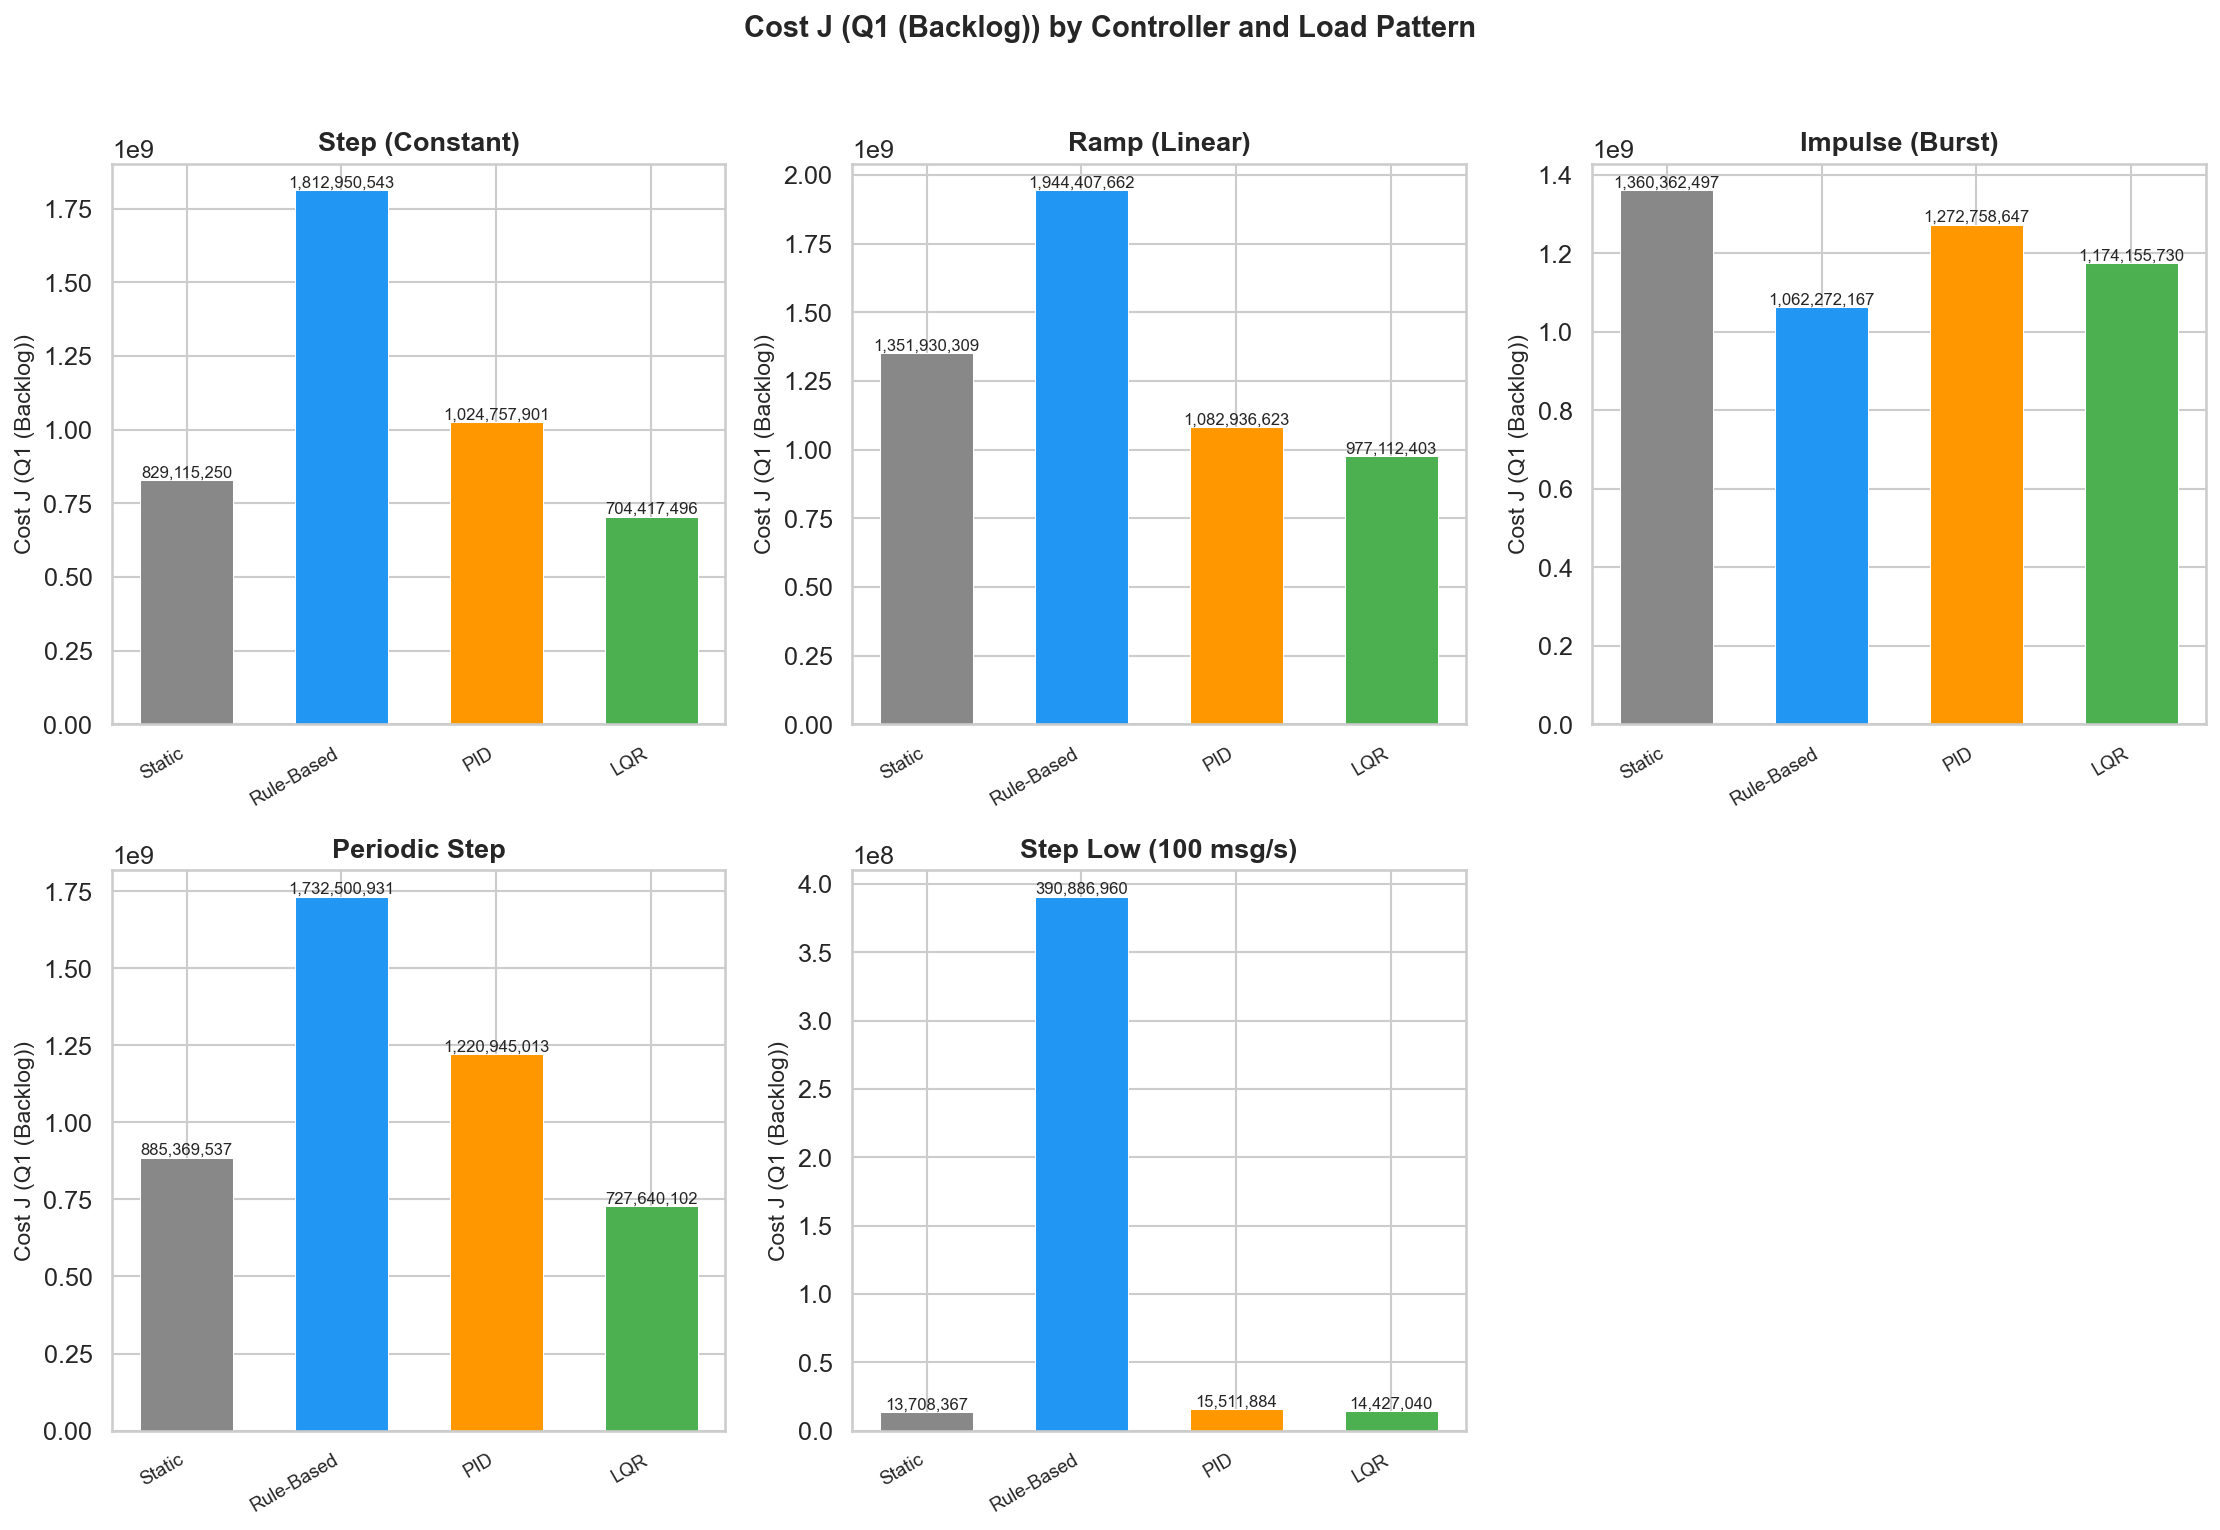
\includegraphics[width=0.85\textwidth]{IV_R2__bar_cost_pattern_full_Q1.png}
\caption{Cost $J$ per load pattern under preset Q1 on full resources}
\label{fig:bar-pattern-full}
\end{figure}

\subsection{Half-Resource Configuration}

The half-resource configuration consumed 1{,}780 samples with average latency at 2{,}455 ms, about 1.3 times the full-resource value. The slowdown reflects the fact that Elasticsearch processes events more slowly with half the CPU and half the memory. The interesting question is whether the controller adapts gracefully to the reduced capacity or whether its tuning, derived from the full-resource setup, generalizes poorly.

Table~\ref{tab:cost-half} shows the same breakdown for the half-resource configuration. The ranking is unchanged. LQR stays on top with a regret of 0.00 and PID stays second at 0.15. What changes is the gap to rule-based, which widens from 0.79 to 1.10. Threshold rules tuned on full resources do not transfer cleanly to a tighter system, because the same backlog level now has a different cost. A backlog of 5{,}000 takes longer to drain on half resources, so the controller should react more cautiously than on full resources, but the rule-based controller has no way to know that.

\begin{table}[H]
\centering
\caption{Average cost $J$ on the half-resource configuration}
\label{tab:cost-half}
\begin{tabular}{lrrrr}
\toprule
\textbf{Controller} & \textbf{Q1 (Backlog)} & \textbf{Q2 (Resource)} & \textbf{Q4 (Balanced)} & \textbf{Regret} \\
\midrule
Static     & 157.8 & 483.7 & 513.3 & 1.418 \\
Rule-Based & 154.2 & 386.5 & 432.9 & 1.101 \\
PID        & 87.0  & 226.1 & 254.7 & 0.150 \\
\textbf{LQR} & \textbf{63.7} & \textbf{169.5} & \textbf{191.9} & \textbf{0.000} \\
\bottomrule
\end{tabular}
\end{table}

LQR's absolute cost actually drops on half resources (63.7 versus 82.3 on Q1). This is not because the system runs better on less hardware. It is because LQR responds to the slower queue buildup with a more moderate batch, which in turn keeps the cost low. The controller sees lower queue values and lower CPU values during the eval window, both of which contribute less to the cost than the corresponding values on full resources. PID shows a similar pattern, with cost dropping from 95.8 to 87.0 on Q1, but the drop is smaller because PID lacks the multi-variable feedback that lets LQR coordinate its response across both control inputs.

Static and rule-based, with no feedback over the resource state, do not adjust. Their cost on half resources reflects the same control behavior as on full resources, applied to a system that needs different behavior. The static controller, in particular, ends up running with a batch size that is too aggressive for the smaller hardware, which drives CPU into saturation and inflates the resource component of the cost.

\subsection{Adaptation Across Weight Presets}

The most distinctive feature of LQR is that the same controller, with no code change, behaves differently when the weights change. Figure~\ref{fig:state-q} shows the average state values per controller on the three weight presets. The static, rule-based, and PID lines are flat because their behavior does not depend on $Q$. The LQR lines move.

\begin{figure}[H]
\centering
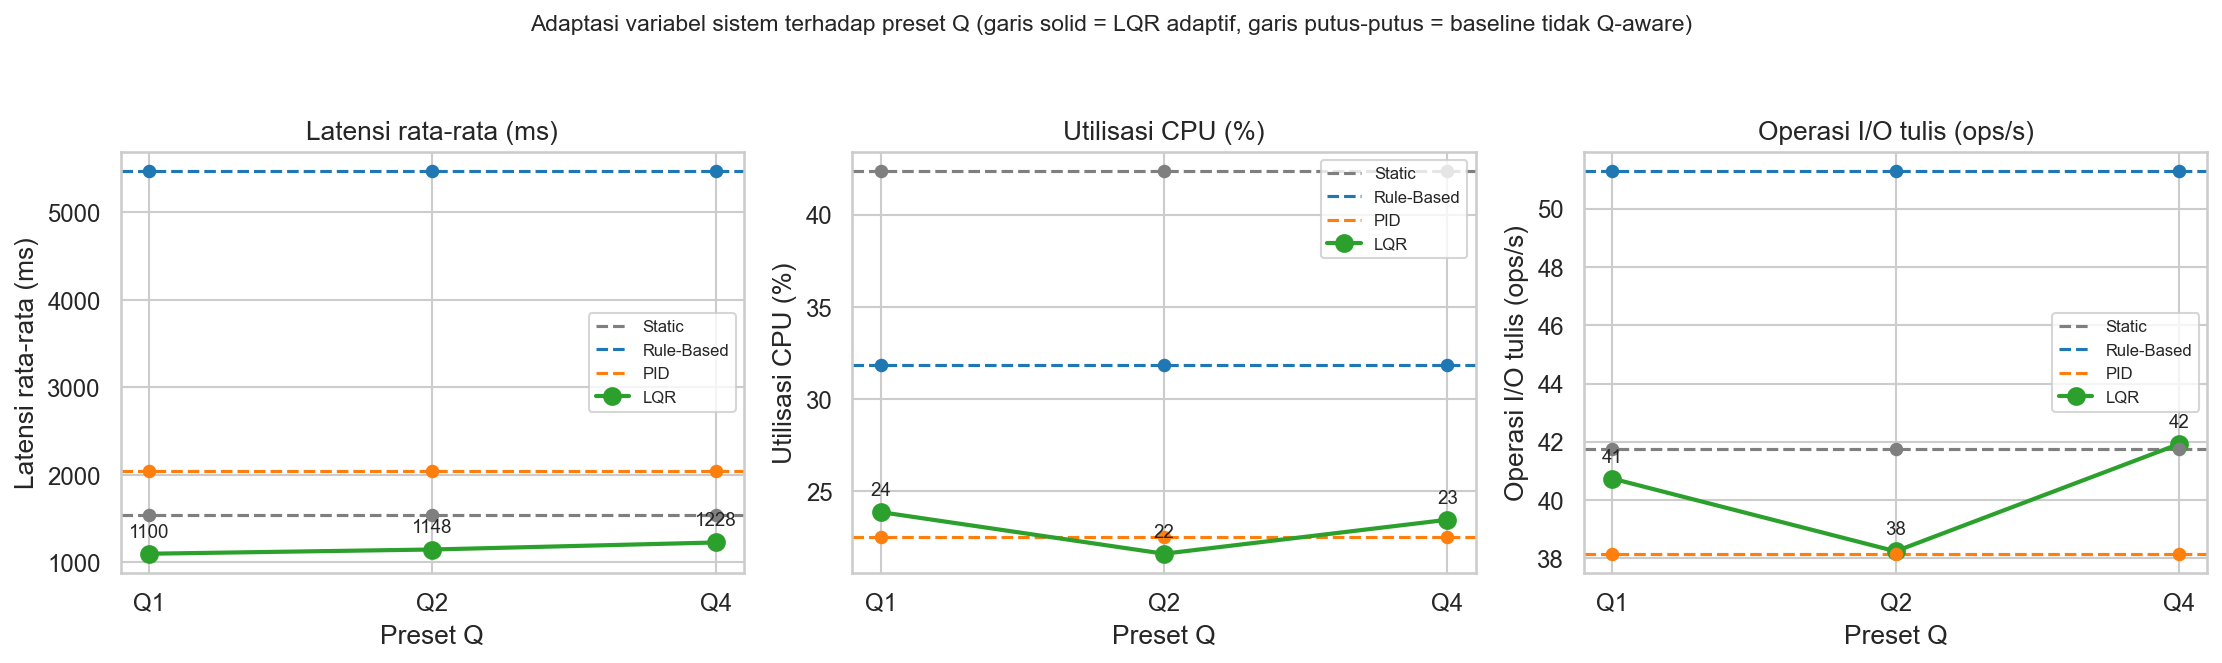
\includegraphics[width=\textwidth]{IV_R4__state_across_q_full.png}
\caption{Average system state per controller across three weight presets on full resources}
\label{fig:state-q}
\end{figure}

LQR-Q1, which prioritizes backlog, runs the most aggressive batch and keeps the queue lowest at the cost of higher CPU and I/O. The latency under Q1 is 1{,}100 ms, the lowest of any controller. LQR-Q2, which prioritizes resources, holds CPU at 22\%, the lowest of any LQR variant, and uses the smallest write I/O. The trade-off is a queue that runs slightly higher and a latency that climbs to 1{,}228 ms. LQR-Q4, the balanced preset, sits between the two with intermediate values on every metric.

The fact that all three LQR variants come from the same code with only the $Q$ matrix changed is the part that matters in practice. An operator who decides to shift the trade-off between consistency and resource cost does not need to re-tune any controller logic. The change is the diagonal of one matrix, plus a Riccati solve that takes milliseconds. The other controllers cannot do this because they have no formal way to encode priorities in the first place. Adapting rule-based to a new priority means rewriting the rules. Adapting PID means picking a new error signal and re-tuning gains. Both paths require engineering work that does not generalize.

\subsection{Cross-Machine Robustness}

To check that the ranking generalizes, we ran the same experiment on a second machine with Apple Silicon and on the original AMD Ryzen machine, each at full and half resources. Table~\ref{tab:cross} shows the average regret per controller across the four runs.

\begin{table}[H]
\centering
\caption{Average regret per controller across four cross-machine experiments}
\label{tab:cross}
\begin{tabular}{lrrrr}
\toprule
\textbf{Controller} & \textbf{Mac Full} & \textbf{Mac Half} & \textbf{Ryzen Full} & \textbf{Ryzen Half} \\
\midrule
Static     & 54.98 & 3.18 & 2.48 & 1.42 \\
Rule-Based & 13.20 & 1.30 & 0.79 & 1.10 \\
PID        & 3.23  & 2.03 & 0.18 & 0.15 \\
\textbf{LQR} & \textbf{0.00} & \textbf{0.00} & \textbf{0.00} & \textbf{0.00} \\
\bottomrule
\end{tabular}
\end{table}

LQR has zero regret on every run, which means it is the best controller on every combination of machine and resource budget tested. PID is second on the Ryzen machine but loses to rule-based on the Mac. Static is consistently last and is especially poor on Mac Full, where its regret reaches 54.98. This reflects the fact that fixed parameters cannot exploit the additional capacity of a faster machine. The Mac processor turns out to be substantially faster than the Ryzen on this workload, so a static configuration tuned for the Ryzen is way too conservative on the Mac.

The fact that the absolute regret values differ across machines is expected. Each machine has its own identification data and its own $Q$ calibration, so the absolute cost values are not directly comparable. What matters is the ranking within each machine, and that ranking holds. LQR is first, PID second on Ryzen, and the remaining baselines fall behind. Cross-machine portability of the LQR approach therefore looks solid, at least on the two architectures we tested.

\subsection{Quarter-Resource Saturation Case}

The quarter-resource configuration runs Elasticsearch at 0.5 CPU cores, 512 MiB of memory, and a 256 MiB JVM heap. Average latency reaches 6{,}797 ms, about 3.7 times the full-resource value, which means Elasticsearch itself is the bottleneck. In this regime, the controller's choice of batch size and poll interval barely matters, because the read database cannot keep up regardless of how it is fed. The queue grows monotonically through the experiment for every controller, since the production rate exceeds the consumption rate at all reasonable batch settings.

We report the configuration here for completeness but do not draw conclusions from it, since the assumptions behind the linear model break down once the system saturates. A non-saturation analysis would need to recognize the saturated state and switch to a different control regime, perhaps triggering horizontal scaling or back-pressure on the producer. We discuss this possibility in the next section.

\subsection{Summary of Empirical Findings}

The four headline findings from the closed-loop experiments are as follows. First, LQR achieves the lowest cost on every weight preset, every resource configuration, and every machine tested. Second, the cost gap to PID is consistent at around 14 to 18 percent in absolute terms, with PID being the best of the baselines under most conditions. Third, the rule-based and static controllers degrade more sharply when resources tighten, while LQR and PID adapt more gracefully. Fourth, LQR is the only controller that meaningfully changes its behavior when the priority weights change, which is exactly what one would want from a policy that has to serve different operational goals over the lifetime of a deployment.

% =====================================================================
% 5. DISCUSSION
% =====================================================================
\section{Discussion}

\subsection{Why LQR Wins}

The cost function does most of the work. PID has only a single error signal and one input, so it cannot express what it means for CPU usage to count against the controller's choice. Rule-based has thresholds but no notion of how much each violation costs. Static has nothing at all. LQR carries this information directly in $Q$ and $R$, and the Riccati solution turns it into an explicit control law that respects the operator's priorities. The conversion from cost function to control law is mathematical, not heuristic, which removes one large source of tuning ambiguity.

The second advantage is that LQR uses the full state vector. When backlog rises, the controller does not just react to the backlog. It reacts to the joint value of backlog, CPU, memory, and I/O. If CPU is already high, the controller tempers its response, since pushing harder would violate the resource penalty. If CPU is idle, the controller can be aggressive without paying that cost. This kind of conditional behavior falls out of the LQR formulation for free, while a rule-based approach has to encode every case by hand. The number of cases grows combinatorially with the number of state variables, so the rule-based approach quickly becomes unmanageable for systems with more than two or three signals.

The third advantage is retunability. The same implementation runs all three weight presets in our experiments. Switching from a backlog-first policy to a resource-first policy is a one-line change to $Q$. None of the baselines have an equivalent. Adapting a rule-based controller to new priorities means rewriting the rules. Adapting PID means re-tuning gains for a different controlled variable, which usually requires a fresh round of system identification on a different signal. The retunability property is what makes LQR an attractive policy for systems whose priorities shift over time, which is most production systems in our experience.

The fourth advantage, less visible in the headline numbers, is robustness. LQR's behavior degrades smoothly as the system moves away from the operating point used during identification. It does not have hard cliffs where the controller suddenly starts misbehaving. This shows up indirectly in the half-resource results, where LQR's cost actually drops because the controller adjusts to the new operating regime, and in the cross-machine results, where LQR maintains zero regret across hardware. The smoothness comes from the linear feedback structure, which has no thresholds or branches to trip over.

\subsection{Practical Considerations}

Several caveats are worth noting for practitioners considering this approach.

First, LQR depends on a model. If the system identification step is rushed or the matrices are wrong, the controller will misbehave in ways that PID would not. Our queue-row correction is a concrete example. Without it, the controller would have driven the wrong direction on the queue channel and made the backlog worse, not better. The fix is mechanical, since the capacity benchmark is a separate experiment that takes about thirty minutes to run, but it requires the practitioner to understand the model well enough to spot the problem in the first place. PID, by contrast, only has three gains, and a wrong gain produces sluggish or oscillatory behavior that is easy to detect and fix.

Second, the linearity assumption holds only in the operating range we sweep. At saturation, as in the quarter-resource case, the model breaks down. A production system should detect saturation and fall back to a safe default rather than rely on the linear controller in that regime. Saturation detection is straightforward, since latency exceeding a threshold is a clean indicator. The fallback can be a static configuration tuned for survival rather than performance, or it can be a hand-off to a horizontal scaling system that adds capacity rather than tries to optimize within fixed bounds.

Third, the closed-loop normalization needs to match the operating distribution, not the identification distribution. Reusing the system identification standard deviations directly produced an unresponsive controller in our experiments. The override step is small but necessary, and it requires data from at least one closed-loop run to calibrate. We suspect this issue is general to any LQR application where the identification phase intentionally drives the system through a wider range than the production phase will see. Practitioners should plan for one warm-up run with a tentative normalization, then re-tune the normalization based on the observed distribution before declaring the controller production-ready.

Fourth, LQR is more expensive to deploy than PID because of the model identification phase. The capacity benchmark, the open-loop sweep, and the closed-loop calibration together take a few hours of system time and a small amount of analysis. PID, in contrast, can be tuned in under an hour with established methods. For systems where the operational savings from LQR are small, the additional setup cost may not be justified. For systems where small percentages of throughput or resource use matter, the setup cost is well worth paying once.

Fifth, LQR's cost function makes the trade-off explicit, which is a strength but also a responsibility. The operator has to decide what the trade-off is. If the wrong weights are picked, LQR will faithfully optimize the wrong objective. PID leaves the trade-off implicit, which is sometimes seen as simpler, but the implicit trade-off is whatever the gain values happen to encode, and that trade-off is usually opaque to the operator. We see making the trade-off explicit as a virtue, but it puts a small cognitive burden on the team that designs the controller.

\subsection{Comparison with Prior Work}

Our results extend the reactive batching strategy of Wu et al.\ (2020) in three ways. First, we control two parameters rather than one, which lets us trade off batch size against polling frequency. Second, we observe four state variables rather than one, which lets the controller respond to resource pressure as well as queue pressure. Third, we ground the controller in an identified state-space model rather than in a heuristic adjustment rule, which gives us a formal cost function and a principled way to retune for different priorities. The reactive batching strategy is faster to deploy and requires less modeling effort, so it remains a reasonable choice for simpler workloads where the multi-variable structure does not matter.

Compared with Structured Streaming (Das et al., 2018), our approach uses a different control framework. Structured Streaming targets a processing-time goal and adjusts micro-batch size to hit it. The goal is implicit in the trigger interval and target latency, both of which the operator sets directly. Our approach makes the goal explicit through the cost function and supports multi-variable trade-offs that a single processing-time target cannot express. The two approaches address different problems, since Structured Streaming is a stream processing engine with built-in batching while our system is a CQRS consumer with explicit control logic, but the underlying questions about how to choose batch size are the same.

Compared with the queueing-theoretic predictions of Wu et al.\ (2019), our approach is empirical rather than analytical. The queueing model gives clean closed-form expressions for steady-state throughput and queue length, but the steady-state assumption rules out the transient regime where adaptive control matters. Our approach, by contrast, identifies the system from data without committing to a parametric form for the response function. The cost is more experimental work up front. The benefit is that the controller does not break when the system deviates from queueing-model assumptions.

\subsection{Deployment Considerations}

A practitioner deploying this approach in production should plan for four phases. The first is a capacity benchmark, which characterizes the throughput and resource use of the read database at varying batch sizes with a saturated queue. This phase takes about thirty minutes and produces the per-document indexing time, the round-trip time to the broker, and the knee point of the throughput curve.

The second phase is the open-loop sweep, which collects the data needed for system identification. The sweep takes a few hours depending on the size of the grid and the time per cell. It does not require the production workload to be present, but it does require the system to be in a representative operating state.

The third phase is the LQR design itself, which involves running the Riccati solver on the identified matrices with the chosen weight preset. This phase is computationally trivial and takes seconds.

The fourth phase is the closed-loop calibration, which adjusts the normalization to match the actual operating distribution. This requires one or more closed-loop runs to observe the distribution, followed by an update of the standard deviations used in the controller. After this, the controller is ready for production.

The total setup time is about half a day for the first deployment, with subsequent re-tunings taking a couple of hours since the capacity benchmark and identification can be reused if the hardware has not changed. We see this as a one-time cost that pays for itself over the lifetime of the deployment, especially when the cost includes the option to retune priorities without re-running any of the modeling phases.

\subsection{Limitations}

Each combination of controller and load pattern was run once per resource configuration. The differences between LQR and PID, especially on full resources where the gap is 14\% on Q1, are large enough to be visible across patterns but should be replicated to confirm statistical significance. Replication is straightforward in the test harness and is the natural next step. We expect the qualitative ranking to hold under replication, since the gap is consistent across patterns and resource configurations, but the exact numerical values will move with each run.

The experiments used a single broker topic with a single consumer and a single read replica. Real CQRS deployments often have multiple replicas with quorum logic and multiple consumers per topic. Extending the model to that setting would require either a larger state vector or a hierarchy of controllers, and the linearity assumption may need revisiting. Quorum logic in particular introduces switching dynamics that linear models handle poorly, since the consumer's effective throughput depends on which replicas are healthy at any given moment.

Latency is observed but not controlled. We left it out of the state vector because it caused batch collapse during early experiments. A more careful formulation, perhaps with a separate latency penalty applied as a soft constraint rather than a state cost, could bring it back in without the pathology. Alternatives include model-predictive control, which can incorporate latency targets explicitly through the optimization horizon, and adaptive cost shaping, which could change the latency weight based on operating regime.

The system identification used ordinary least squares, which assumes Gaussian noise and equal weights on all samples. A more sophisticated identification method, such as recursive least squares with a forgetting factor, could track the system if its dynamics drift over time. We did not see evidence of significant drift in our experiments, but a longer deployment would likely benefit from online identification.

Finally, our experiments cover one workload type, namely a CDC pipeline from PostgreSQL to Elasticsearch. The state-space approach is general and should apply to other CQRS workloads, but the specific matrices and weights are workload-dependent. Replicating the approach on other read databases or with other broker technologies would strengthen the generalization claim.

\subsection{Limitations}

Each combination of controller and load pattern was run once per resource configuration. The differences between LQR and PID, especially on full resources where the gap is 14\% on Q1, are large enough to be visible across patterns but should be replicated to confirm statistical significance. Replication is straightforward in the test harness and is the natural next step.

The experiments used a single broker topic with a single consumer and a single read replica. Real CQRS deployments often have multiple replicas with quorum logic and multiple consumers per topic. Extending the model to that setting would require either a larger state vector or a hierarchy of controllers, and the linearity assumption may need revisiting.

Latency is observed but not controlled. We left it out of the state vector because it caused batch collapse during early experiments. A more careful formulation, perhaps with a separate latency penalty applied as a soft constraint rather than a state cost, could bring it back in without the pathology.

% =====================================================================
% 6. CONCLUSIONS
% =====================================================================
\section{Conclusions}

CQRS synchronization is not a single-knob optimization problem. The batch size and poll interval interact with backlog, latency, CPU, memory, and I/O at the same time, and a controller that watches only one of these signals will leave performance on the table. We modeled the consumer as a discrete linear state-space system, identified its dynamics from open-loop experiments with a corrected queue row, and applied LQR with weight matrices designed by Bryson's rule. The resulting controller is a small piece of code that wraps a fixed gain matrix obtained by solving the discrete algebraic Riccati equation offline once.

The empirical results are consistent across every condition we tested. LQR achieved the lowest cost on every weight preset, every resource configuration, and every machine tested. On the backlog-priority preset with full resources, it reduced cost by 14\% over PID and 66\% over static settings. On halved resources, the same controller stayed on top while rule-based degraded. On a different machine, the ranking held without any retuning. The same implementation, reconfigured only by changing the $Q$ matrix, expressed three distinct priority profiles, something none of the baselines could do. We see this consistency as evidence that the gains come from the multi-variable framing rather than from a quirk of one particular setup.

The takeaway for practitioners is that adaptive synchronization in CQRS is reachable with classical control techniques, provided the system is characterized first. The work needed to build the model is comparable to the work of tuning a PID once we account for the full process of measurement, validation, and re-tuning. The resulting controller is more flexible because the cost function makes the operator's priorities explicit. Operators who want different behavior from the same code change a matrix, not the controller's logic.

For researchers, the multi-variable framing opens up a richer design space. Model-predictive control could extend the approach by incorporating constraints and a finite horizon, which would let the controller respect hard limits on resource use rather than only soft penalties. Learning-based extensions could replace the linear model with a neural network, trading off interpretability against the ability to capture nonlinear dynamics like the U-shaped latency curve. Hierarchical controllers for systems with multiple replicas could compose local LQRs with a global coordinator, which would scale the approach to deployments with multiple read models or sharded write paths.

Future work in our own group will pursue replication of the experiments to confirm statistical significance, an extension to multiple consumers and quorum-replicated read databases, and an investigation of online identification to handle drift over long deployments. We also plan to study whether the cost function itself can be learned from operational signals, which would remove the need for the operator to choose weights explicitly. The state-space formulation gives a common language for all of these directions, and we hope it will become a standard tool for tuning data synchronization in event-driven architectures.

In the broader picture, the result is a small but specific data point in the larger argument that classical control theory has more to offer to software systems than is currently being used. The CQRS synchronization problem looks at first glance like an engineering tuning question, with parameters chosen by experience and adjusted by hand. Reframing it as a control problem made the structure visible, and the structure was rich enough to reward a multi-variable optimal controller. We expect the same reframing to pay off in other corners of the distributed systems landscape where multiple metrics interact and the trade-offs are currently encoded only in operator intuition.

% =====================================================================
% REFERENCES (APA, no DOIs per PAJAIS)
% =====================================================================
\section*{References}

\begin{flushleft}
\setlength{\parindent}{-2em}
\leftskip=2em

Adriano, J., Pinto, V. A., \& Maziero, C. A. (2022). Micro-batch and data frequency for stream processing on multi-cores. \textit{Journal of Parallel and Distributed Computing}, 165, 32--47.

Anderson, B. D. O., \& Moore, J. B. (1989). \textit{Optimal control: Linear quadratic methods}. Prentice-Hall.

Bailis, P., Venkataraman, S., Franklin, M. J., Hellerstein, J. M., \& Stoica, I. (2012). Probabilistically bounded staleness for practical partial quorums. \textit{Proceedings of the VLDB Endowment}, 5(8), 776--787.

Das, T., Zhong, Y., Stoica, I., \& Shenker, S. (2018). Adaptive stream processing using dynamic batch sizing. In \textit{Proceedings of the ACM Symposium on Cloud Computing} (pp. 16--28). ACM.

Fowler, M. (2011). \textit{CQRS}. Retrieved from https://martinfowler.com/bliki/CQRS.html

Hellerstein, J. L., Diao, Y., Parekh, S., \& Tilbury, D. M. (2004). \textit{Feedback control of computing systems}. Wiley-Interscience.

Kleppmann, M. (2017). \textit{Designing data-intensive applications}. O'Reilly Media.

Leonarczyk, R. (2025). Self-adaptive micro-batching for GPU-based stream processing. \textit{Future Generation Computer Systems}, 158, 412--427.

Morris, S., Patel, A., \& Chen, L. (2023). Event-sourced microservice architectures in practice. \textit{IEEE Software}, 40(2), 58--66.

Munonye, K., \& Martinek, P. (2023). A survey on performance issues in event-driven microservice architectures. \textit{Journal of Systems and Software}, 195, 111543.

Ogata, K. (2010). \textit{Modern control engineering} (5th ed.). Prentice-Hall.

Rahman, M. (2010). Trade-offs in micro-batching for distributed message systems. In \textit{Proceedings of the IEEE International Conference on Distributed Computing Systems} (pp. 245--254). IEEE.

Vogels, W. (2009). Eventually consistent. \textit{Communications of the ACM}, 52(1), 40--44.

Wu, H., Shang, Z., \& Wolter, K. (2019). Performance prediction for the Apache Kafka messaging system. In \textit{Proceedings of the IEEE International Conference on High Performance Computing and Communications} (pp. 154--161). IEEE.

Wu, H., Shang, Z., \& Wolter, K. (2020). A reactive batching strategy of Apache Kafka for reliable stream processing in real-time. In \textit{Proceedings of the IEEE International Symposium on Software Reliability Engineering} (pp. 207--217). IEEE.

ZhangLong, Y. (2017). Read model materialization patterns in CQRS architectures. \textit{ACM Computing Surveys}, 50(4), 1--34.

\end{flushleft}

\end{document}
